\newpage
\fancyhead[C]{Rory Millard}
\section{Project Financing} \label{financing}

% --- Introduction: Clearer statement of purpose ---
This section presents an economic analysis comparing the drone-based landmine detection system proposed in this report with legacy manual metal-detector methods, focusing on the cost-effectiveness for surveying \textbf{and demining} operations near Kharkiv, Ukraine. The metric for comparison is the total cost to survey and clear one square kilometre (km²) of land. The analysis quantifies the system's financial improvement over the legacy system, and links it to the sensor performance metrics (Precision $P_{sys}$ and Recall $R_{sys}$).


\subsection{Comparative Cost Structures} \label{subsec:cost_structures}


Legacy demining operations involve a technical survey costing $C_\text{legacy survey}=$ \$305,000 per km², and a subsequent clearance phase, with a nominal cost of $C_\text{clearance}=$ \$2,940,000 per km² \footnote{\url{https://kse.ua/wp-content/uploads/2023/09/Mining-brief_Final-1.pdf}}. However, manual technical surveys typically result in clearing only half the surveyed area, implying an effective precision improvement of 2$\times$ over 'blind', indiscriminate clearance. This is significantly lower than the 27.7$\times$ suggested in Section \ref{fusion_bounds}. The operational cost for legacy surveying and disposal is estimated as:

\begin{equation*}
C_{\text{legacy}} = \$305,000 + (0.5 \times \$2,940,000) = \$1,775,000 \text{/km}^2 
\end{equation*}


The drone-based system proposed in this report replaces the manual technical survey. The operational survey cost is significantly lower, estimated at $C_\text{survey}=$ \$300 per km² for approximately 10 hours of flight time per 1~km$^2$. To compare the two systems, it is assumed that the \textit{cost of investigating and clearing a flagged region just depends on its total area}. The total landmine clearance cost for the drone system $C_{\text{drone}}$ therefore is dependent on the number of points flagged, which is a function of the system's precision and recall, as detailed in Section \ref{subsec:performance_savings}. Table \ref{tab:cost_comparison_structured} provides a breakdown of the estimated operational costs.

\begin{table}[h!]
% Removed \small command
\centering
\caption{Structured Cost Comparison: Drone System vs. Legacy Manual Team (Kharkiv Case Study - USD Figures, 5-Year Amortization)}
\label{tab:cost_comparison_structured}

\begin{tabular}{lcc} 
\toprule
\textbf{Operational Costs} & \textbf{Drone System} & \textbf{Legacy System} \\
\midrule
\multicolumn{3}{l}{} \\
Technical Survey Cost (\$/km²) & \$300 & \$305,000 \\ 
Time for Technical Survey (days/km²) &  5 & 10 \\ 
Flags / Area Needing EO Clearance & 3.6\% & 50\% \\ 
Cost of EO Clearance (\$/km²) & \$106,000 & \$1,470,000 \\
Time for EO Clearance (days/km²) & [Missing Data - depends on flags] & [Missing Data] \\ \addlinespace
\textbf{Total Time to Demine 1 km² (days)} & \textbf{10} & \textbf{20} \\ \addlinespace
\textbf{Total Cost to Demine 1 km² } & \textbf{\$117,700} & \textbf{\$1,775,000}  \\
\bottomrule
\end{tabular}
\end{table}

\subsection{Performance-Linked Financial Savings} \label{subsec:performance_savings}

The operational cost of the proposed system depends on the number of point flagged for mine clearance. This depends on the initial mine density $\rho_0$, and the system's precision $P_{sys}$ and recall $R_{sys}$. 

The fraction of land $A_\text{flagged}$ flagged for mine clearance is:
\begin{equation}
A_{\text{flagged}} = \frac{\text{Area Flagged}}{\text{Total Area}} \approx  \frac{\rho_0 R_\text{sys}}{P_\text{sys}}. 
\label{eq:flags_fraction} % Renamed label for clarity
\end{equation}
Given the assumption of constant cost for clearing a flagged area, the total operational cost for the drone system per km² $C_{\text{drone}}$ is:
\begin{equation}
C_{\text{drone}}(P_\text{sys}, R_\text{sys}) = C_{\text{survey}} + A_{\text{flagged}} \times C_{\text{clearance}} 
\approx \$300 + \left( \frac{\rho_0 R_\text{sys}}{P_\text{sys}} \right) \times \$2,940,000 
\label{eq:drone_op_cost} % New label
\end{equation}



Equation \ref{eq:drone_op_cost} demonstrates that improving $P_{sys}$ results in a large operational cost reduction by reducing the number of points flagged for mine removal. While maximizing recall $R_{sys}$ is important for safety (as discussed in Section \ref{lossmatrix}), achieving high precision is the only way the system can be economically viable. The cost savings by choosing the proposed system over legacy systems are plotted in Figure \ref{fig:financial_savings} as a function of $P_\text{sys}$ and $R_\text{sys}$. The expected region of system performance is also plotted (using the bounds from Section \ref{fusion_bounds}), indicating an \textbf{expected operational cost saving of between $\approx$ \$1.65~m - \$1.75~m per km²} surveyed, over the legacy operational cost of \$1.775~m/km². 


% --- Figure - Needs updated caption reflecting source of data/need for recalc ---
\begin{figure}[h!]
\centering
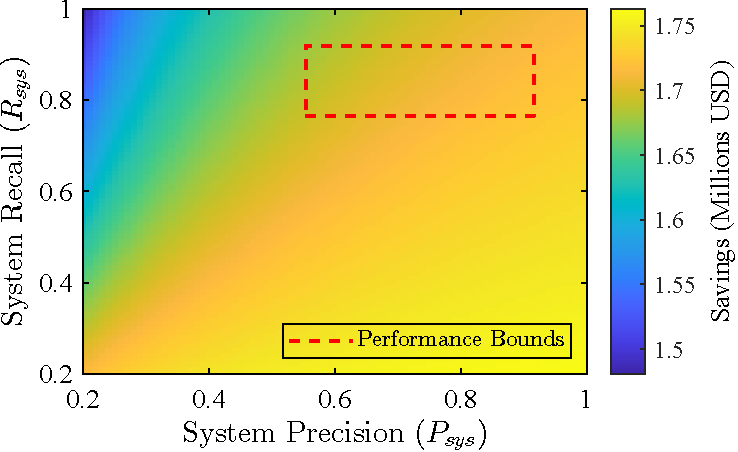
\includegraphics[width=0.5\textwidth]{figs/Rory/financial_savings.pdf} 
\caption{Operational cost savings of the proposed system over legacy systems for surveying and demining, varying with $P_{sys}$ and $R_{sys}$s.}
\label{fig:financial_savings}
\end{figure}

% --- NEW FIGURE/TABLE SUGGESTION GOES HERE ---
% See suggestion below

% --- Conclusion: Rewritten for stronger synthesis ---
\subsection{Conclusion} \label{subsec:finance_conclusion}

This economic analysis of operational costs strongly suggests that the proposed drone-based landmine detection system offers substantial financial advantages over traditional manual methods. Key drivers include drastically reduced technical survey costs (\$300 vs \$305,000 per km²) and potentially lower overall personnel and operational expenditures.

\paragraph{Future Work} The ultimate cost-effectiveness is intrinsically linked to the system's detection performance, especially its precision $P_{sys}$. As demonstrated, higher precision directly translates to lower operational clearance costs by reducing the number of false positives requiring investigation (Equation \ref{eq:drone_op_cost}). 
\begin{enumerate}
    \item Fixed and operational costs, validated from other sources
    \item Confirm with a YOLO model trained on better data that, and tested on real-world experiments, that these precisions and recalls can be achieved. 
    \item Investigate the lifespan of the drone system and discount wear and tear as an operational cost to get a better picture of the financial picture.
\end{enumerate}

Achieving the target performance metrics will solidify the system's financial viability, potentially enabling humanitarian organizations to significantly increase the area cleared within existing budgets, thereby amplifying the project's impact.